%% \documentclass[a4paper]{article}
\documentclass[12pt]{article}

%% Language and font encoding
\usepackage[english]{babel}
\usepackage[utf8x]{inputenc}
\usepackage[T1]{fontenc}

\usepackage{tgtermes} % times font

%% Sets page size and margins
\usepackage[a4paper,top=3cm,bottom=2cm,left=3cm,right=3cm,marginparwidth=1.75cm]{geometry}

%% Useful packages
\usepackage{amsmath}
\usepackage{graphicx}
\usepackage[colorinlistoftodos]{todonotes}
\usepackage[colorlinks=true, allcolors=blue]{hyperref}
\usepackage[useregional]{datetime2}
\usepackage{array}
\usepackage{tabularx}
\usepackage{natbib}
\usepackage{authblk}



\title{Evaluation of Community Detection Algorithms}
\author{Ping-Chang Lee}
\affil{MSc in Data Science \& Statistics \\ The University of Bath}
\date{{September}{2022}}

\begin{document}

\maketitle
\pagebreak

%% Access Page 1
    
\bigbreak\bigbreak\bigbreak
\bigbreak\bigbreak\bigbreak
\bigbreak\bigbreak\bigbreak

This dissertation may be made available for consultation within the University Library and may be photocopied or lent to other libraries for the purposes of consultation.
\bigbreak\bigbreak\bigbreak
Singed: ***My Signature Here***
\pagebreak


\tableofcontents
\pagebreak

\section{Introduction}
In recent decades, the study related to network analysis has drawn the attention of scholars form various fields. Among numerous topics of network analysis, discovering the community structure of network is one of the most essential approach to learn the complicated systems that can not easily be cracked by solely conducting shallow researches\cite{1}. 

\bigskip

Despite there are dozens of community detection algorithms already implemented to real-world network analysis and have already granted great success in many fields \cite{2,3}, the sample networks for performance testing are often simplified and sparse. In this dissertation, the LFR benchmark graph is introduced to mock the real-world network by increasing the complexity of the network. Afterwards, a subset of community detection algorithms are applied to the artificial network. Due to the nature of algorithms, the dissertation will introduce the computation complexity and their procedures. Also, since some algorithms are iterative, the dissertation selects the best result from iterations for evaluations under different circumstances. Next, the dissertation provides a series of approaches to evaluate the partitions of algorithms. As mentioned, a network can have either high complexity or very sparse structure, there is no consistent classification yet to determine if a given partition of a network is 'good'. The dissertation particularly underline the methodology on goodness of partition and the measure of similarity between the partition of a community detection algorithm and the ground truth community partition(network that is already labeled by communities).

\section{Background}
\subsection{Network Structure}

In general, there are two basic components that construct a network. A network(or a graph) G is composed by V and E, where V is the vertex(node) set containing all the vertices that belongs to the network and E is the edge(relation) set containing all the edge between vertices if two are connected. Further properties can be added to the network if the network is weighted or directed. In order to fit the goals of this dissertation, the label function L is add to the network, that is $G = \{V,E,L\}$. $L(v_i) = c_j$ indicates vertex $v_i$ belongs to community with label of $c_j$. With the definition of label stated previously, the community $C_i$ can be defined as $C_i = \{ L(v) = c_i \text{, } \forall v \in V \}$. 
Furthermore, given a partitioned network with n communities, let $C_i$ be the community with a label of $c_i$, then 
$\bigcup_{1 \leq i \leq n} C_i \subseteq V(G)$. The data structure of a network is beneficial for graph analysis since the researchers can solely work on the relation of vertices and edges without considering the whole space.

\bigskip


\begin{figure}
\centering
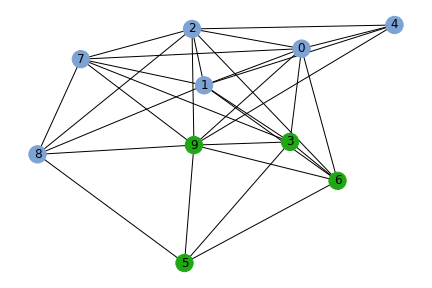
\includegraphics[width=0.5\textwidth]{fig_1.png}
\caption{\label{fig:fig_1}A network with unique ID and color labels. In this network, there are two communities whose nodes are either colored in sky blue or in grass green.}
\end{figure}


\subsection{Community}

In network analysis, community in a network often refers to a group of vertex that has closer relation comparing to other vertices that are not in the same group. To simplify the complexity of the context, in this dissertation, no vertex will be assigned to multiple communities, that is $\forall C_i,\ C_j \text{, } i \neq j$, $C_i \cap C_j = \phi$. Depending on the content of network, such as social network, chemical network, and ecosystem network, the definition of forming a community may vary. Furthermore, if given a weight network such as a geographical network, we can intuitively determine if vertices can be grouped into a community by taking their distance(weight of edges) into consideration. Directed network can also be partitioned into communities if the community detection is designed carefully with the help of linear algebra and information theory\cite{4}. Without doubt, there are networks that has no intention of creating communities such as random graphs or Barabási–Albert model\cite{5}; researchers can still apply community detection algorithms to unveil the latent structure from these networks.

\pagebreak
\begin{thebibliography}{100}

\bibitem{1}
  
    \textit{Community detection algorithms: A comparative analysis},
    Lancichinetti, A. and Fortunato, S.,2009.
    1986.
  
\bibitem{2}
    \textit{Parallel Protein Community Detection in
    Large-scale PPI Networks Based on
    Multi-source Learning}
    J. Chen, K. Li, K. Bilal, A. A. Metwally, K. Li, and P. S. Yu,
    2018
    
\bibitem{3}
    \textit{Community detection in Social Media. Data Mining and Knowledge Discovery}
    Papadopoulos, S., Kompatsiaris, Y., Vakali, A. and Spyridonos, P.,
    2011
    
\bibitem{4}
    \textit{Quantitative methods for ecological network analysis. Computational Biology and Chemistry}
    Ulanowicz, R.E.,
    2004
    
\bibitem{5}
    \textit{tatistical mechanics of complex networks. Reviews of Modern Physics}
    Albert, R. and Barabási, A.-L.,
    2002

        
\end{thebibliography}

\end{document}